% Illustration and advantages of variable capacity
\begin{slide}[Les PàCCV adaptent leur capacité aux besoins\\
			  pour fonctionner de façon continue]

%\drawhelplines

% Illustration
\only<1->{
\node [anchor=mid west, align=left] at (p5cl cs:1,13) {capacité\\fixe};
\node [anchor=mid west, align=left] at (p5cl cs:1,6) {capacité\\variable};

\begin{scope}[shift={(p5cr cs:1,12)},
			  x=\bigcol/6+\baselineskip/6, y=3\baselineskip]

\draw [semithick] (0,.3333333) -- (3,.33333333) |- (6,.666666);
\draw [col, very thick]
	  (0,0) .. controls (0.1, 1) and (0.2, 1) .. (0.5,1)
   -- (0.5,1) .. controls (0.52, 0) and (0.6, 0) .. (0.7,0)
   -- (1.5,0) .. controls (1.6, 1) and (1.7, 1) .. (2,1)
   -- (2,1) .. controls (2.02, 0) and (2.1, 0) .. (2.2,0)
   -- (3,0) .. controls (3.1, 1) and (3.2, 1) .. (3.5,1)
   -- (4,1) .. controls (4.02, 0) and (4.1, 0) .. (4.2,0)
   -- (4.5,0) .. controls (4.6, 1) and (4.7, 1) .. (5,1)
   -- (5.5,1) .. controls (5.52, 0) and (5.6, 0) .. (5.7,0) -- (6,0);
	
\end{scope}


\node [becomes, rotate=180] at (p5cr cs:2,10) {};


\begin{scope}[shift={(p5cr cs:1,5)},
			  x=\bigcol/6+\baselineskip/6, y=\baselineskip]

\draw [semithick] (0,1) -- (3,1) |- (6,2);
\def\phase{46.87329}  % found numerically with scipy
\draw [col, very thick] plot [domain=0:3, samples=100, smooth]
			(\x, {1 - exp(-2*\x) * cos(700*\x + \phase) / cos(\phase)});
	
\end{scope}


\begin{scope}[shift={($(p5cr cs:1,6)+(\colv+\baselineskip,0)$)},
			  x=\bigcol/6+\baselineskip/6, y=\baselineskip]

% use rect line cap for joining but clip the part sticking out
\clip (p5cr cs:1,6) rectangle ++(2\colvsep,3\baselineskip);
\def\phase{46.87329}
\draw [col, very thick, line cap=rect]
	plot [domain=0:3, samples=100, smooth]
			(\x, {1 - exp(-2*\x) * cos(700*\x + \phase) / cos(\phase)});
\end{scope}
}

\node [becomes, rotate=180, visible on=<2>] at (p5cr cs:2,4) {};

\node [anchor=base west, visible on=<2>] at (t5cr cs:1,0) {
	\begin{minipage}[b]{2\colvsep}
	\begin{listed}
		\item Opère à basse température
		\item COP saisonnier plus élevé
	\end{listed}
	\end{minipage}};

%% Advantages
%\node (N1) [anchor=base, align=left, visible on=<2->]
%	at ($(t5cl cs:2,12)+(\colv/2,0)$)
%	{Et ainsi elles permettent d'éviter un fonctionnement intermittent};
%\node (S1) [anchor=base west, align=left, visible on=<2->]
%	at ($(N1.base west)-(0,5\baselineskip)$)
%	{Il y a une meilleure\\performance saisonnière};
%\node (P1) [anchor=base, align=left, visible on=<2->]
%	at ($(S1.base)-(0,5\baselineskip)$)
%	{La consommation globale\\est réduite};
%\node (S2) [anchor=base east, align=left, visible on=<3->]
%	at ($(N1.base east)-(0,5\baselineskip)$)
%	{Les échangeurs sont dimensionnés\\pour des conditions extrêmes};
%\node (P2) [anchor=base, align=left, visible on=<4>]
%	at ($(S2.base)-(0,5\baselineskip)$)
%	{La plage de température\\est plus large};
%\node [becomes, rotate=180, visible on=<2->]
%	at ($(N1.south -| S1)!0.5!(S1.north)$) {};
%\node [becomes, rotate=180, visible on=<2->]
%	at ($(S1.south)!0.5!(P1.north)$) {};
%\node [becomes, rotate=180, visible on=<3->]
%	at ($(N1.south -| S2)!0.5!(S2.north)$) {};
%\node [becomes, rotate=90, visible on=<3->]
%	at ($(S1.east)!0.5!(S2.west)$) {};
%\node [becomes, rotate=180, visible on=<4>]
%	at ($(S2.south)!0.5!(P2.north)$) {};
%\node [becomes, rotate=90, visible on=<4>]
%	at ($(P1.east)!0.5!(P2.west)$) {};

\end{slide}





% Étude de cas
\begin{slide}[Un modèle dynamique adéquat est nécessaire\\
			  pour simuler correctement les PàCCV]

\node [anchor=base west] (text) at (t5cl cs:0,4) {
	\begin{minipage}[b]{\dimexpr2\colvsep+4\quanta}\raggedright
		\emph{Exemple}\\[2\baselineskip]
		Simuler le profil de consommation\\
		d'une unité de résidence typique,\\~\\
		avec un pas de temp $ \Delta t = \SI{1}{\minute} $
	\end{minipage}};

\node [anchor=south east] at (p5cr cs:4,3)
	{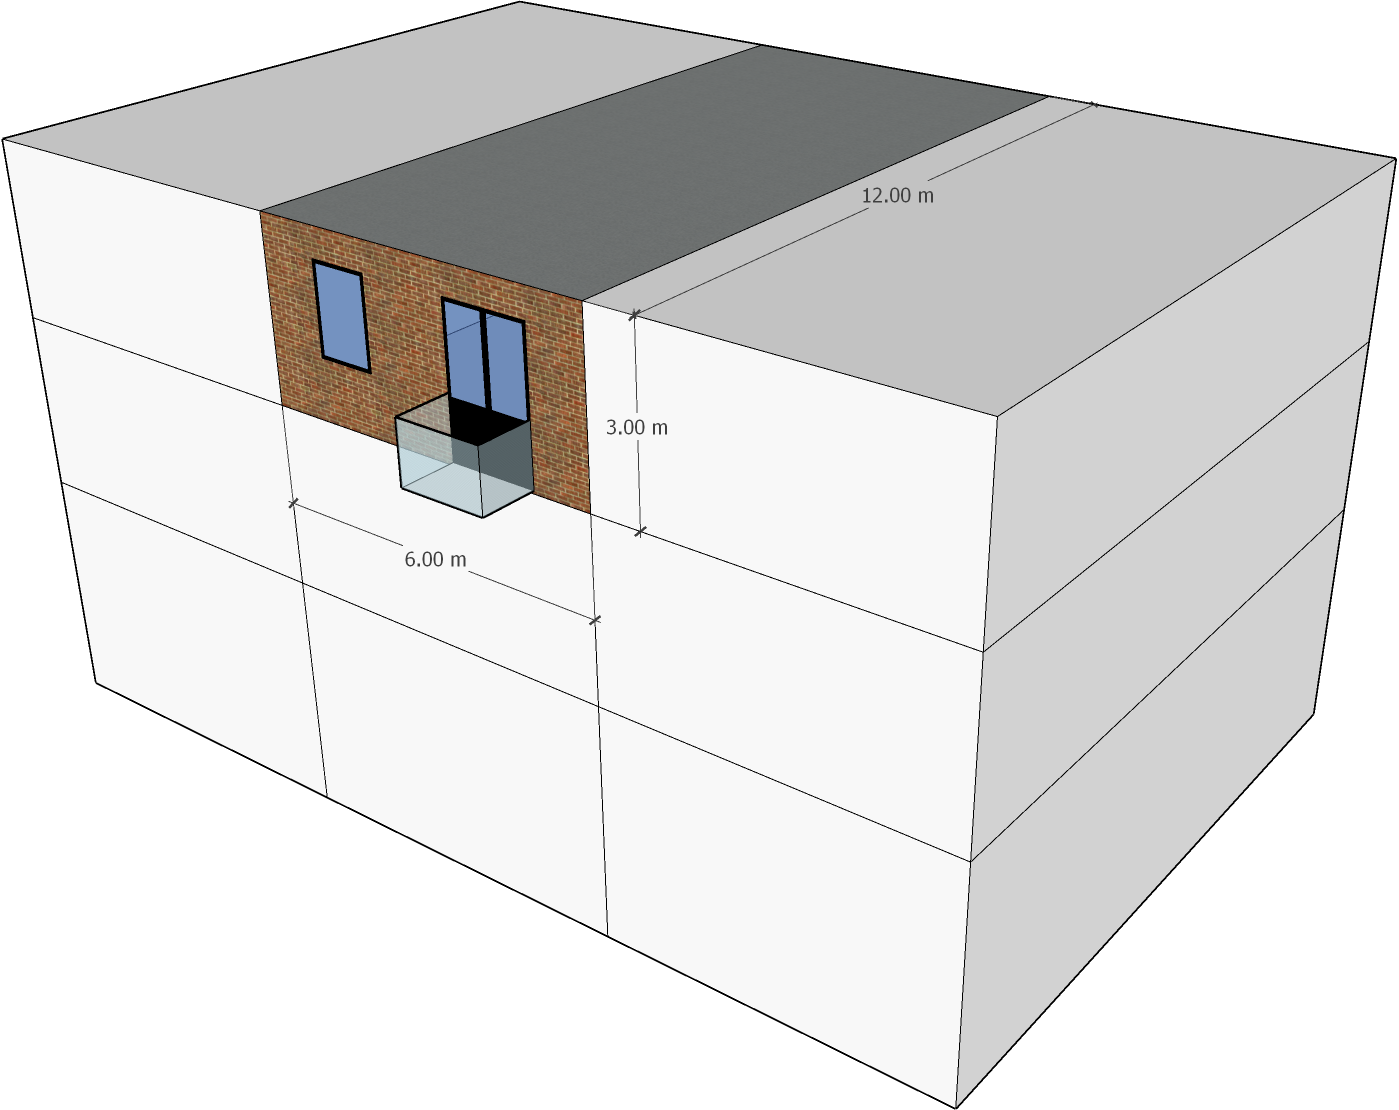
\includegraphics[height=9\baselineskip]{pictures/plex-unit}};

\end{slide}





% Ductless mini-split
\begin{slide}[On se concentre sur des PàCCV air-air,\\
			  de type mini-split]

\node (pic) [anchor=south west] at (p5cr cs:1,1.5)
	{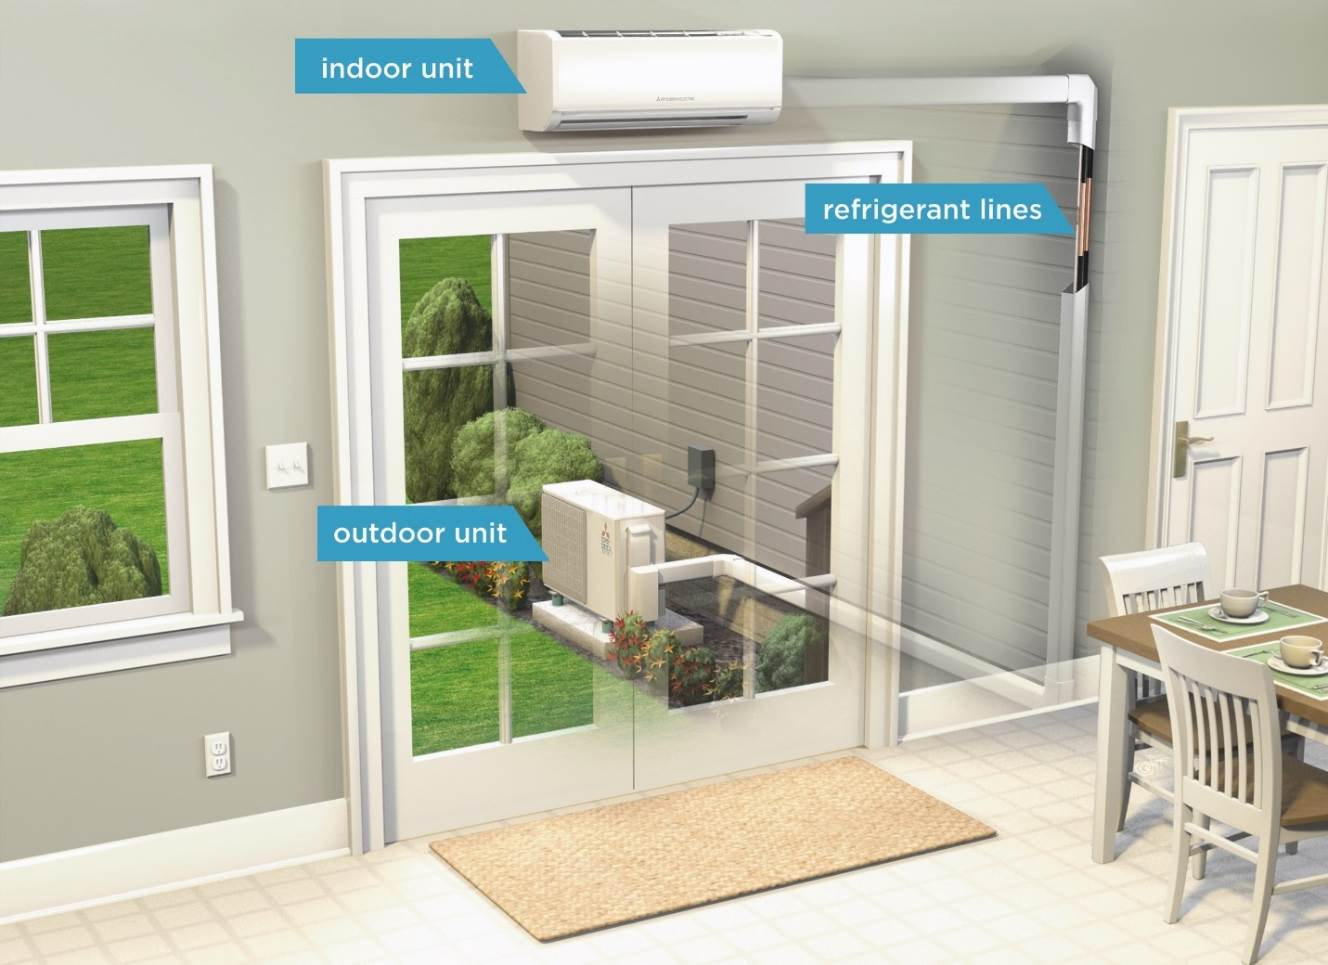
\includegraphics[width=3\colvsep]{pictures/mini-split}};
\node[yshift=-\quantum, anchor=north west] at (pic.south west)
	{\scalebox{.3}{\textcopyright{} ENERGY STAR}};


\begin{scope}[shift={($(p5cl cs:0,5)+(.2,-.2)+(.6pt,0)$)}]

% air flux
\path [draw=white, line width=1mm, -{Triangle[scale=0.7]},
	   shade path={left color=col!30, right color=col}]
	   (.2,3.4) .. controls (.2,3.3) and (.2,2.55) .. (.5,2.25)
	   .. controls (.8, 1.95) and (1.3,1.95) .. (1.4,1.95);
\node (r) [above, yshift=1mm] at (.2,3.4) {$r$};
\node (s) [right, xshift=1mm] at (1.4,1.95) {$s$};
\node [above right, yshift=2mm, gray] at (.5,2.25) {\Va};

% indoor unit
\filldraw [gray!50, very thick] (0,3) rectangle (-.2,2);
\draw [dotted] (0,3) -- (0.5,3);
\draw [very thick, line cap=rect] (.5,3) -- (1,3)
	node [right, align=left, font=\footnotesize,
		  shift={(2\quantum,-2\quantum)}] {unité\\intérieure}
	to [out=270, in=60] (.9,2.3)
	(0,3) |- (0.5,2) -- ++(340:.2)
	(.75,2.15) -- ++(340:.2);

\end{scope}

% outdoor unit
\begin{scope}[shift={($(p5cl cs:0,1.5)+(.2,0)+(\quantum+1ex,0)$)}]

\path [draw=white, line width=1mm, -{Triangle[scale=0.7]},
	   shade path={left color=col, right color=col!30}]
	(-.2,1.1) -- (1.5,1.1);
\node [anchor=east, xshift=-\quantum] at (-.2,1.1) {$o$};

\fill [gray!50] (-.6pt,0) rectangle ($(1,.2)+(.6pt,0)$);
\draw [very thick] (0,0.6) -- (0,.2) -| (1,0.6)
				   (1,1.8) |-
				   node [right, align=left, font=\footnotesize,
		  				 shift={(2\quantum,-2\quantum)}]
		  		   {unité\\extérieure} (0,2.2) -- (0,1.8);
\draw [thick, dotted] (0,1.7) -- (0,0.7);
\draw [thick] foreach \y in {0.7, 0.9, ..., 1.7}{(.9,\y) -- (1.1,\y)};

\end{scope}

\end{slide}





% Données incomplètes
\begin{slide}[Les manufacturiers ne donnent pas suffisamment\\
			  d'informations sur les performances%
			  \only<5->{, ni sur le contrôle}]

\only<1>{
\begin{axis}[plot options, clip=false,
			 at={(p5cl cs:2,2)},
			 width=\bigcol+2\baselineskip, height=12\baselineskip,
			 xtick={-26.1, 15},
			 xticklabels={\num{-26.1}\phantom{$-$},
			 			  \phantom{\,\si{\celsius}}\SI{15}{\celsius}},
			 ytick={1.42, 4.75},]
\foreach \i in {1, ..., 4}{
	\addplot [mark=*, mark size=1pt, semithick] table[x=Toa, y=COP_at_T\i]
		{data/manu-data-heating.tsv};}
\foreach \i/\COP in {1/4.75, 2/4.524, 3/4.339, 4/3.961}{%
	\edef\temp{\noexpand\node (T\i) at (axis cs:15,\COP) {};}
	\temp}
\end{axis}
\node [anchor=mid west, font=\footnotesize] at (p5cl cs:1,14) {COP};
\node [anchor=base east, font=\footnotesize] (Toa)
	at (t5cr cs:4,0) {\To};
\foreach \i/\Ti in {1/15.6, 2/18.3, 3/21.1, 4/23.8}{
	\node [font=\footnotesize, gray, anchor=east] (Tr\i)
		at (T\i -| Toa.east) {\SI{\Ti}{\celsius}};
	\draw [gray] (T\i)++(4.5pt,0) -- ($(Tr\i.west)-(4pt,0)$);}
\node [anchor=west, yshift=-2\baselineskip, gray, font=\footnotesize]
	at (Tr4.west) {\Tr};
}

\def\displayat{2}
\foreach \row/\rowlabel in {0/3, 1/2, 2/1}{
	\foreach \col/\collabel in {2/1, 3/2, 4/3}{
		\colorlet{background}{gray!10}
		\ifnum \row=2
			\ifnum \col=2
				\temporal<3>{
					\colorlet{background}{gray!10}}{
					\colorlet{background}{gray!10}}{
					\colorlet{background}{col!20}}
			\fi
		\fi
		\ifnum \col=2
			\renewcommand\displayat{2}
		\else
			\renewcommand\displayat{3}
		\fi
		\begin{axis}[visible on=<\displayat-4>,
					 enlargelimits=false, scale only axis,
					 hide axis,
					 at={($(p5cl cs:\col,0)+(0,56*\row*\quantum/3)$)},
					 width=\colv, height=11\baselineskip/3,
					 axis background/.style={fill=background}]
		
		\foreach \i in {1, ..., 4}{
			\addplot [mark=*, mark size=.5pt] table [x=Toa, y=COP_at_T\i]
				{data/manu-data-heating.tsv};}
			
		\end{axis}
		\ifnum \row=0
			\node [xshift=.5\colv, anchor=base, visible on=<3-4>]
				at (p5cl cs:\col,14){\Va[\collabel]};
		\fi
	}
	\pgfmathparse{2+\row}\let\labelypos\pgfmathresult
	\node [anchor=east, visible on=<2-4>] (row\row)
		at ($(p5cr cs:1,0)+(0,{(22+56*\row)*\quantum/3})$)
		{\fc[\rowlabel]};
}

\node[anchor=base] (pct) at ($(t5cl cs:0,6)!0.5!(row1.base west)$)
	{$ {\uncover<4>{{\color{col}1}\above 0.4pt} \uncover<3-4>{3 \times 3}}
	   \uncover<4>{\approx \SI{11}{\percent}} $};

\uncover<3-4>{
	\node [align=left, font=\footnotesize] (required)
		at (pct.202 |- row0) {paires $ (f,\skew{3}\dot V) $\\nécessaires};
	\draw (pct.202)++(0,-4pt) -- ($(required.north)+(0,4pt)$);}
\uncover<4>{
	\node [align=left, font=\footnotesize] (provided)
		at (pct.158 |- row2) {paire $ (f,\skew{3}\dot V) $\\fournie};
	\draw [col] (pct.158)++(0,4pt) -- ($(provided.south)-(0,4pt)$);}


\node [anchor=base west, align=left, visible on=<5>] at (t5cr cs:1,2){
	\begin{minipage}[b]{3\colvsep}\raggedright
	\hskip-.8pt Beaucoup de ``cas spéciaux'' sont détaillés,\\~\\
	\begin{listed}
		\item les limites d'opération\\
			  {\footnotesize\color{gray} fréquences minimale et maximale,
			  							 \ldots}
		\item le contrôle des ventilateurs\\
			  {\footnotesize\color{gray} vitesse en fonction
			  							 de la température}
		\item le contrôle du mode d'opération\\
			  {\footnotesize\color{gray} chauffage ou climatisation,
			  							 selon la consigne}
	\end{listed}
	\vskip\baselineskip \hskip-.8pt mais pas le contrôle normal
									de la fréquence 
	\end{minipage}};

\end{slide}





% Assemblage TRNSYS
\begin{slide}[Le modèle est constitué de\\
			  deux composants TRNSYS]

\fill [col!50] (page cs:22.5,-21) rectangle (page cs:32,-31)
			   (page cs:44,-21) rectangle (page cs:52,-31);
\node [anchor=west] at (p5cl cs:0,7)
	{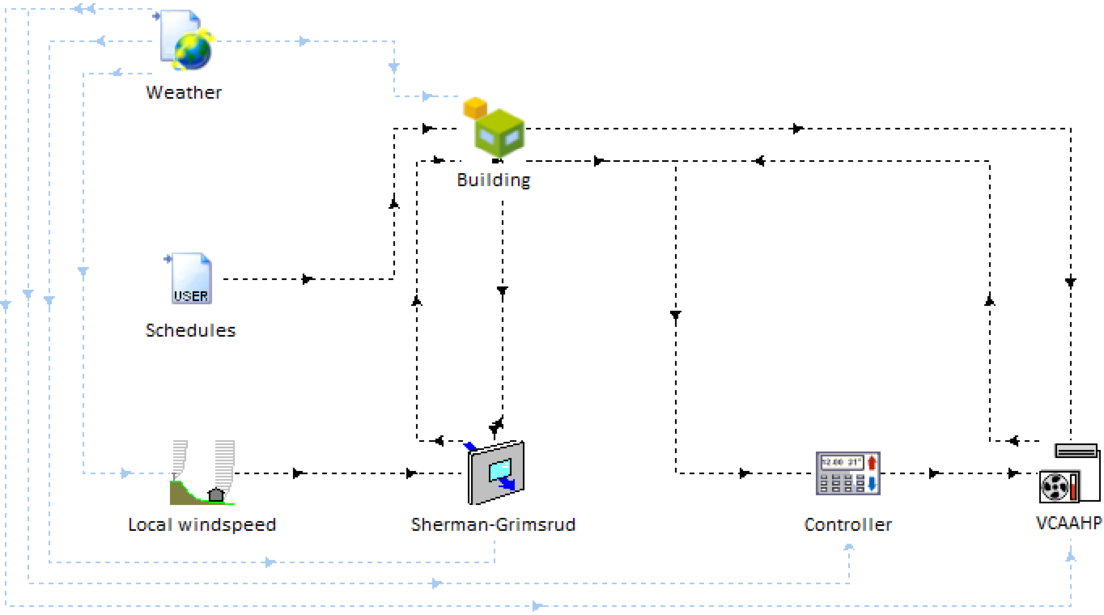
\includegraphics[width=\dimexpr 4\colvsep+\colv-\quantum \relax]
		{pictures/TRNSYS-assembly}};

\end{slide}






\begin{slide}[Les stratégies de contrôle et les performances\\ 
			  sont évaluées expérimentalement]

\node[anchor=north west] at (p5cl cs:.25,15)	{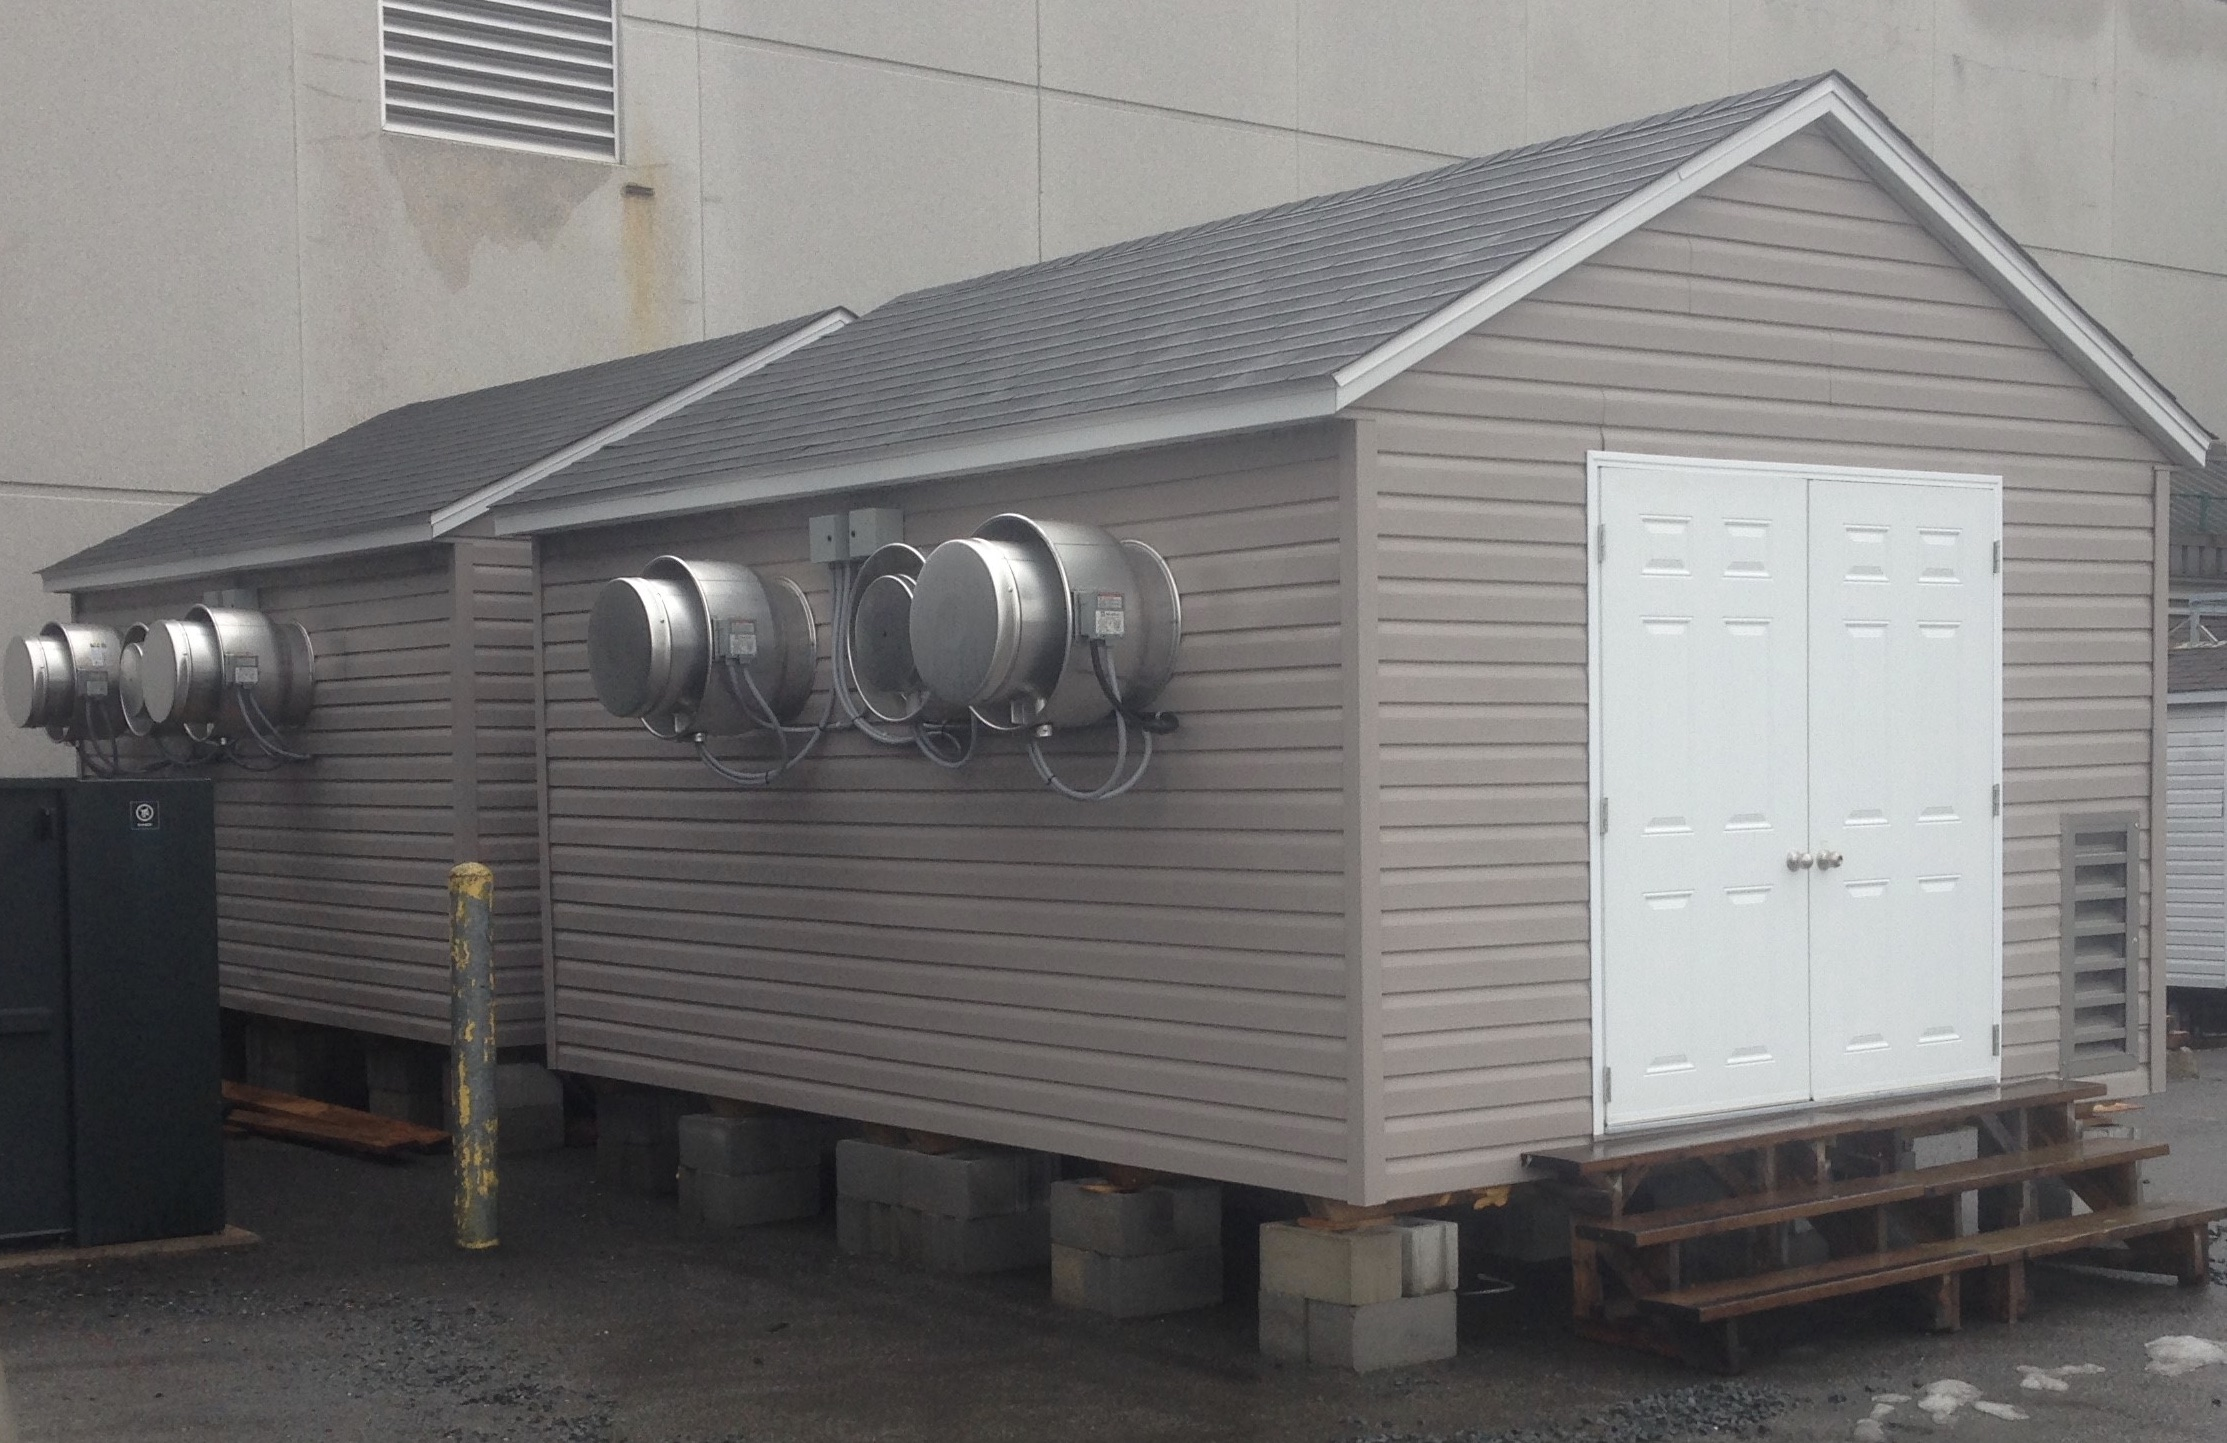
\includegraphics[width=2\colvsep]{pictures/sheds}};
\node[anchor=south west] at (p5cl cs:.25,0)
	{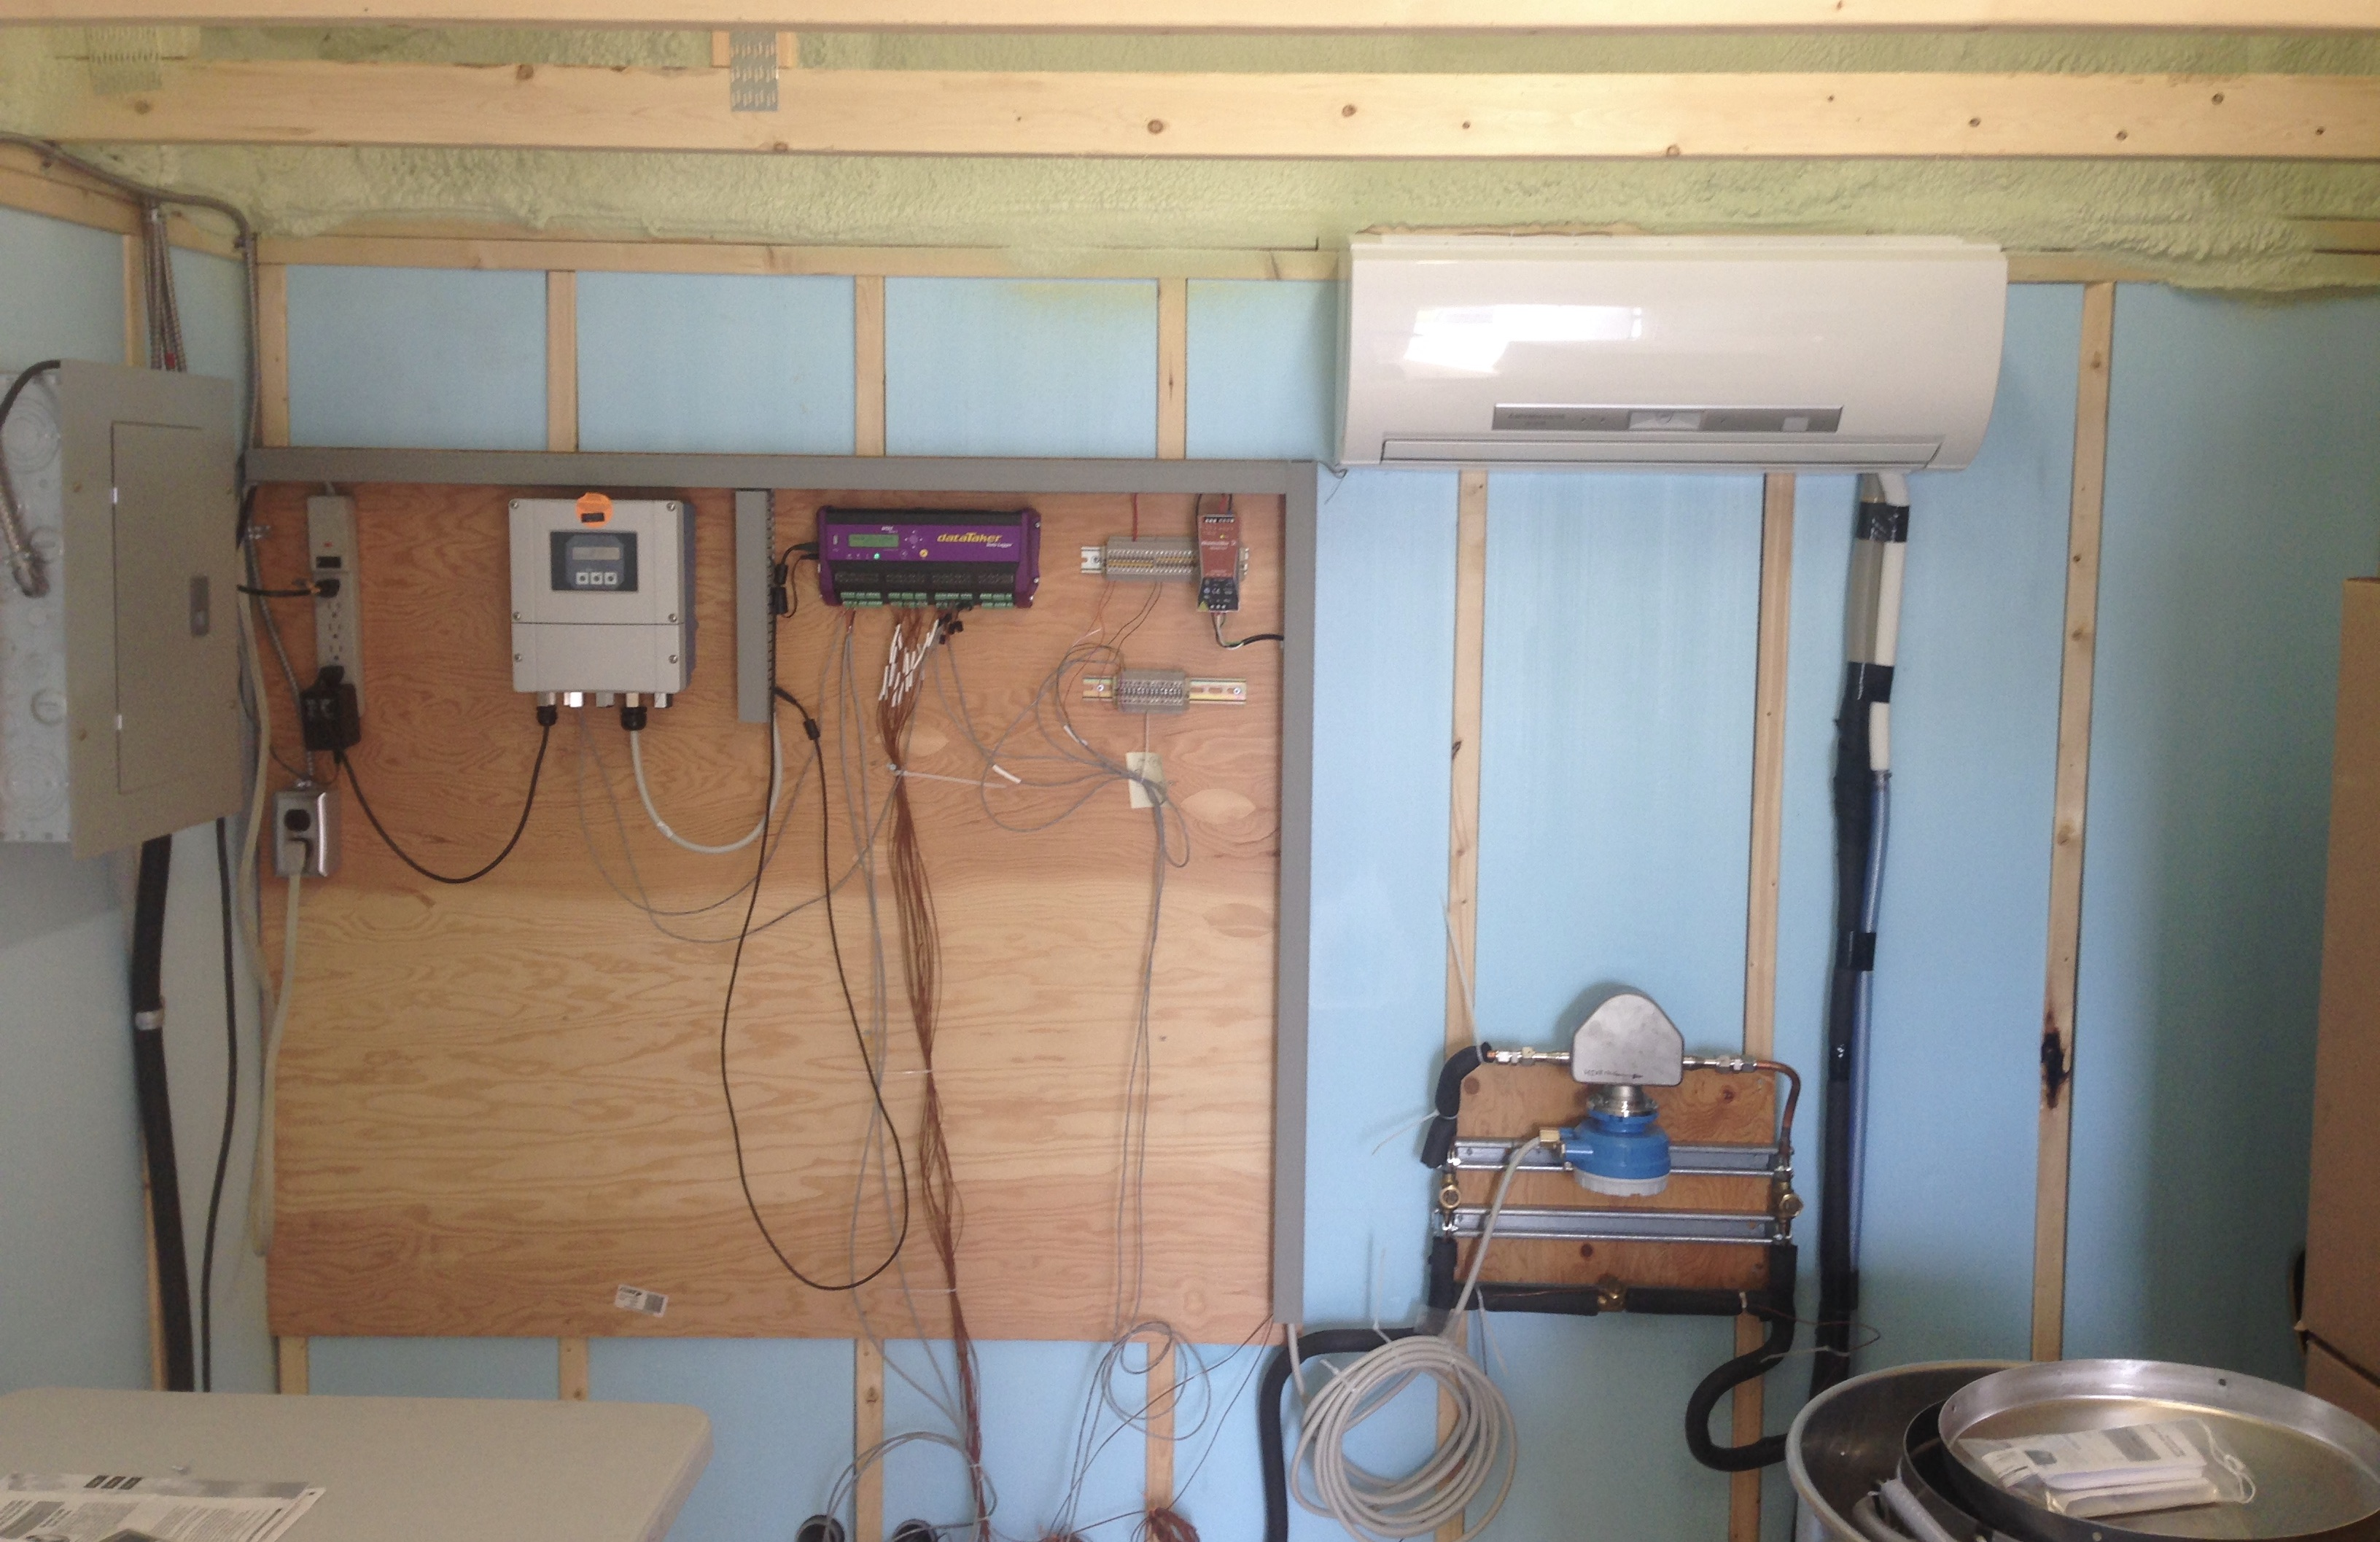
\includegraphics[width=2\colvsep]{pictures/indoor-unit}};
\node[anchor=south east] at (p5cr cs:3.75,0)
	{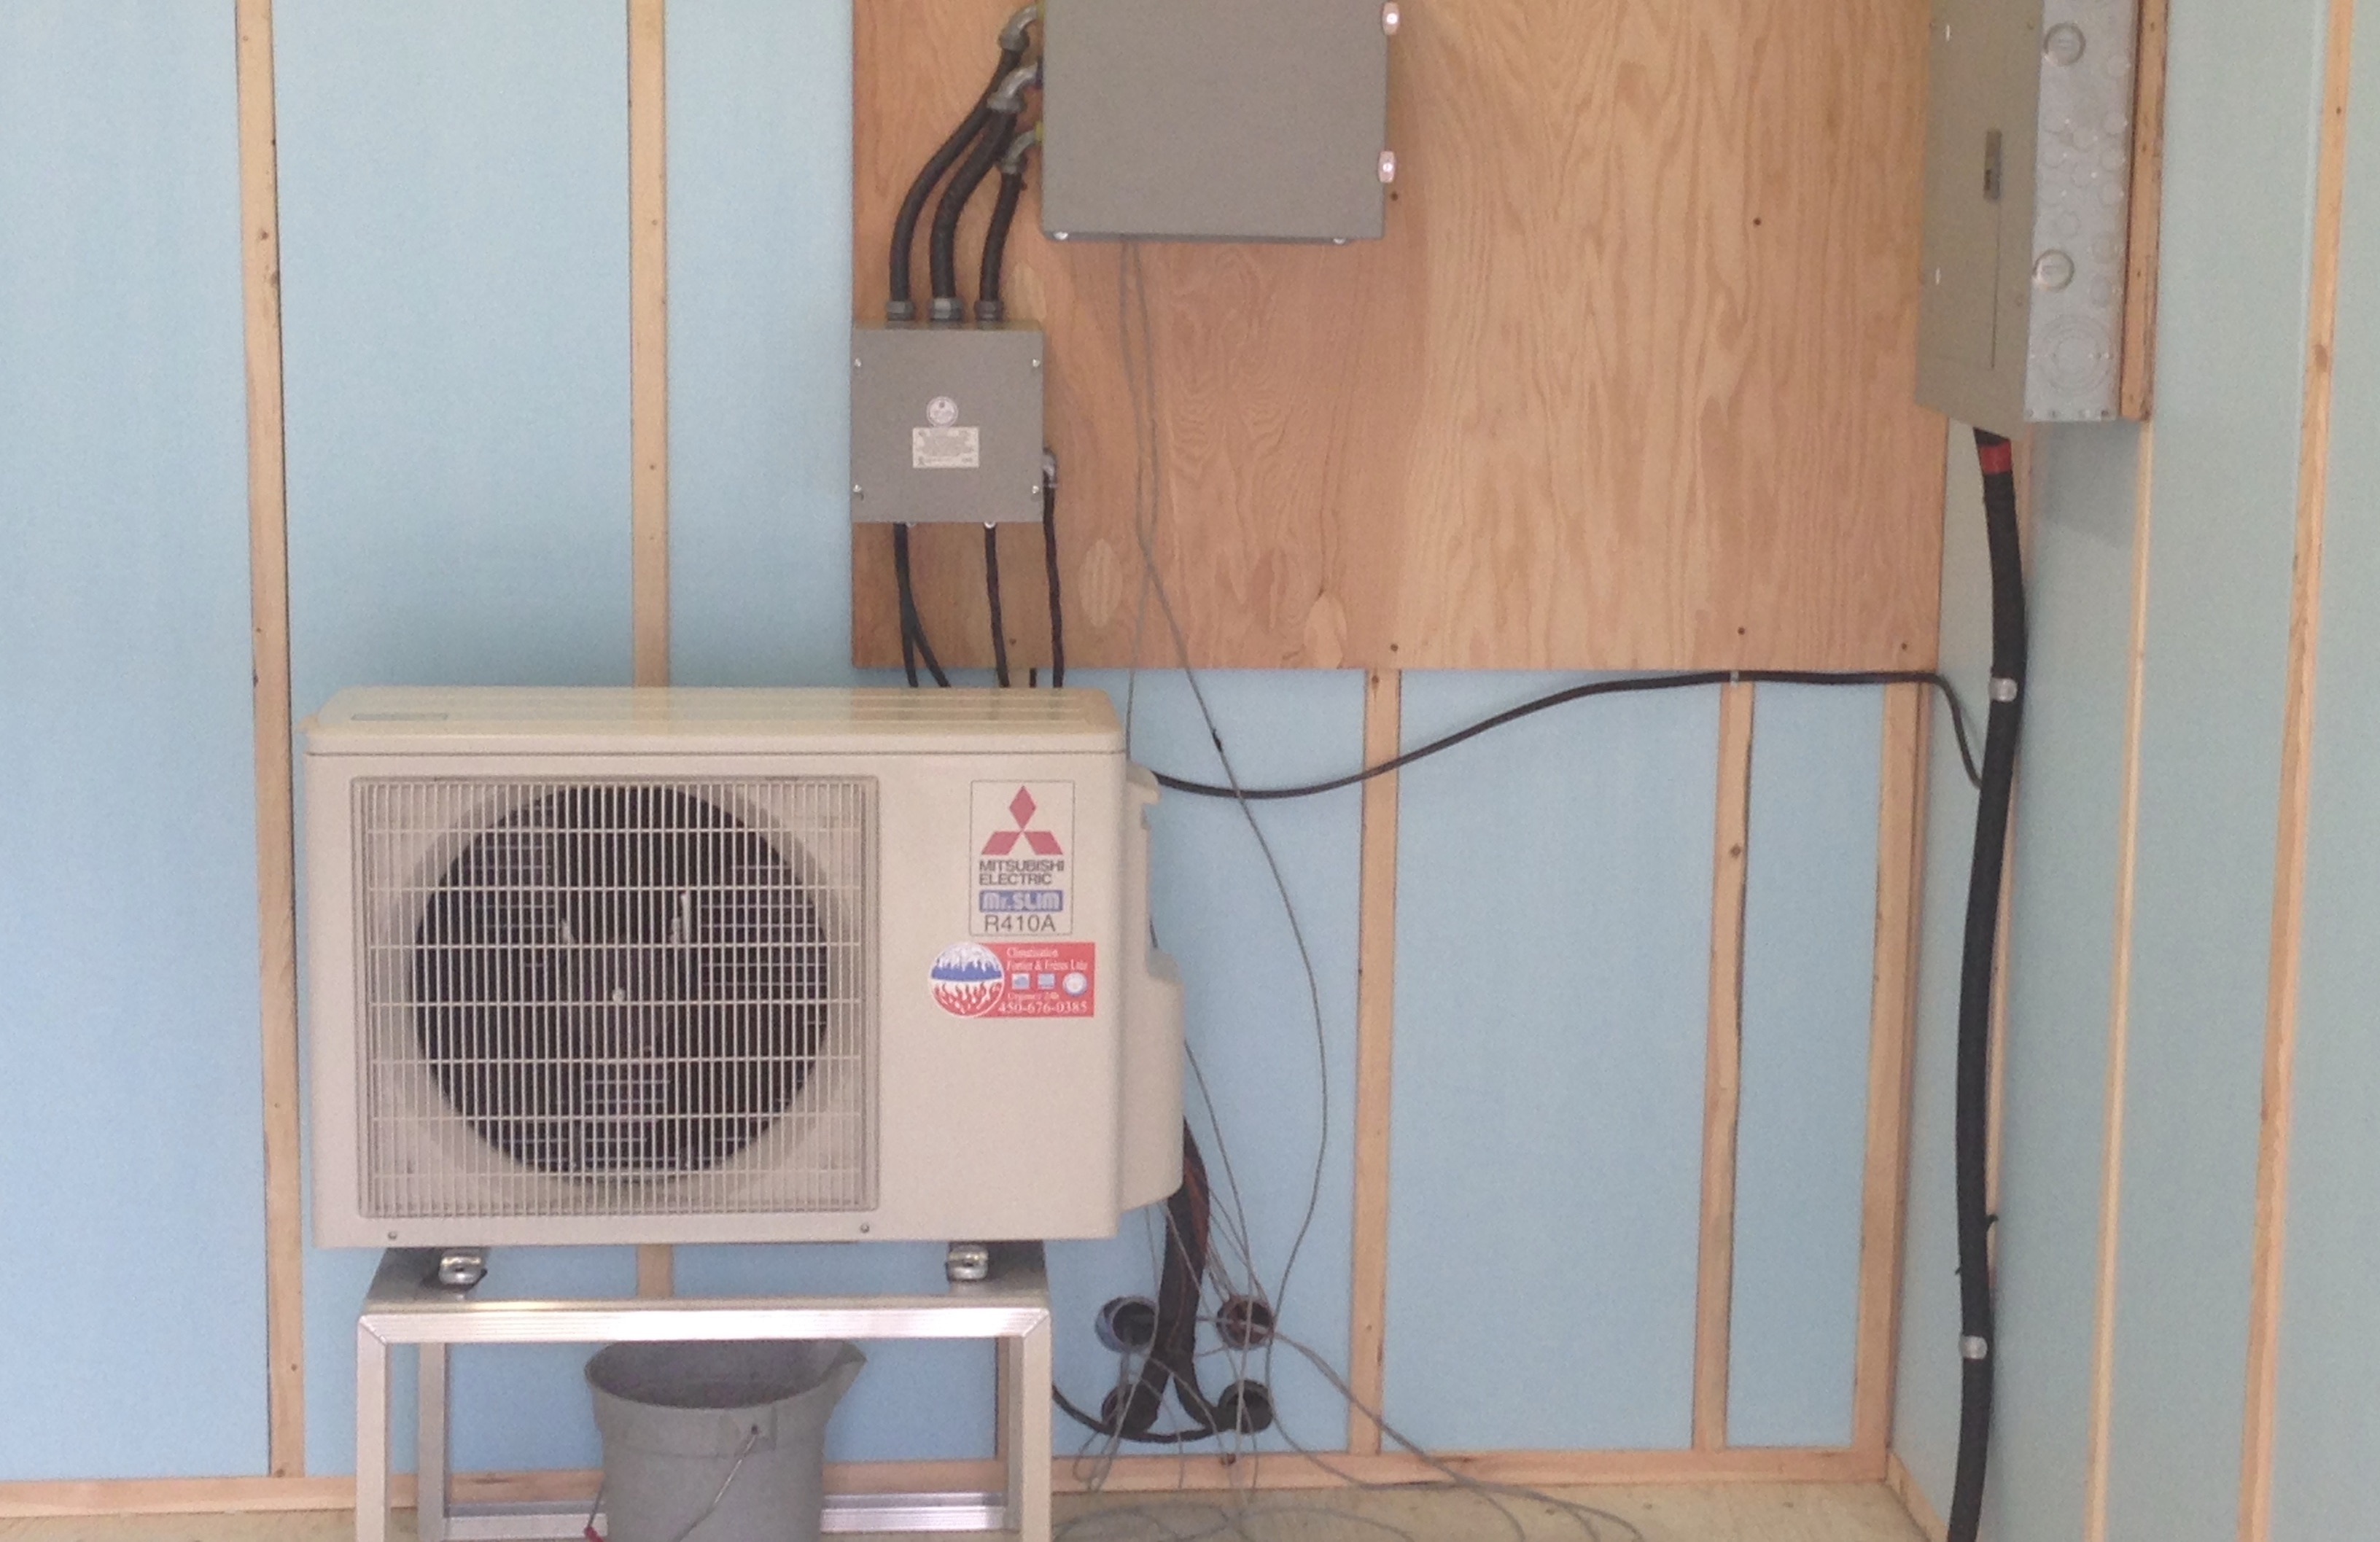
\includegraphics[width=2\colvsep]{pictures/outdoor-unit}};

\node[anchor=base east] at (t5cr cs:3.75,8){
	\begin{minipage}[b]{2\colvsep}
		Pour obtenir les performances dans les conditions désirées,
		\begin{listed}
		\setlength\itemsep{0pt}
			\item la charge
			\item la température extérieure
			\item le débit d'air
		\end{listed}
		sont imposés en contrôlant la quantité d'air entrant
	\end{minipage}};

\end{slide}
